\documentclass[a4paper]{report}
\usepackage[spanish]{babel}
\usepackage[utf8]{inputenc}
\usepackage{graphicx}
\usepackage[document]{ragged2e}
\usepackage{pdflscape}
\usepackage[table]{xcolor}
\usepackage{lscape}
\usepackage{listings}
\usepackage{xcolor}


\lstdefinestyle{mystyle}{
    basicstyle=\ttfamily\footnotesize,
    breakatwhitespace=false,         
    breaklines=true,                 
    captionpos=b,                    
    keepspaces=true,                 
    numbers=left,                    
    numbersep=5pt,                  
    showspaces=false,                
    showstringspaces=false,
    showtabs=false,                  
    tabsize=2
}

\lstset{style=mystyle}

\title{Programa 6 - Automata de Pila}
\author{Leon Tejeda 2CM5}
\date{Enero 2021}

\begin{document}
\maketitle
\begin{flushleft}
INTRODUCCION:

Que es una pila:  Una pila (stack en inglés) es una lista ordinal o estructura de datos en la que el modo de acceso a sus elementos es de tipo LIFO (del inglés Last In First Out, último en entrar, primero en salir) que permite almacenar y recuperar datos.


PLANTEAMIENTO DEL PROBLEMA:

Implementar un automata de pila para reconocer el CFL (Context Free Language o Lenguaje libre de Contexto) {0*n 1*n | n>=1}

Adicionalmente, el programa debe de contar con las siguientes características:

1. La cadena puede ingresar por el usuario o automáticamente.
2. Mandar a un archivo y en pantalla la evaluación del autómata a través de descripciones instantáneas.
3. Animar el autómata de pila.
4. La longitud máxima será manejar cadenas de 100,000 caracteres.

DESARROLLO:

Para este problema se utilizo el lenguaje de C++, para que se viera calramente la implementacion de la pila. Se tuvo que implementar una libreria para que el compilador aceptara el tipo de dato PILA.

El programa solo debia aceptar cadenas de n cantidad de 0's, seguida de n cantidad de 1's, EJ:
0011, 00001111

Si por alguna razon la cantidad de 0's y 1's eran diferente, la cadena sera rechazada, al igual que si estan concatenados, EJ:
010101, 001, 101010

El funcionamiento de la pila seria que cada vez que encontrara un 0, se ingresaria una X dentro de la pila. De lo contrario se sacaria la X de la pila.

Se implemento un menu para ingresar la cadena de manera manual o aleatoria

\newpage

LIBRERIA:

\begin{lstlisting}

#include <iostream>
#include <string>
#include <fstream>
#include <stdlib.h>
#include <time.h>
#include <windows.h>
#include <conio.h>


struct Pila
{
	char dato;
	struct Pila * Siguiente;
	struct Pila * Tope;
	struct Pila * Fin;	
};

struct Pila * Insertar(struct Pila * , char );

void Mostrar_Tope(struct Pila * );

struct Pila * Eliminar_Tope(struct  Pila * );

\end{lstlisting}
\newpage

CODIGO:

\lstinputlisting[language=C++]{Programa6_Automata de Pila.cpp}
\newpage

FUNCIONAMIENTO:

Menu del programa
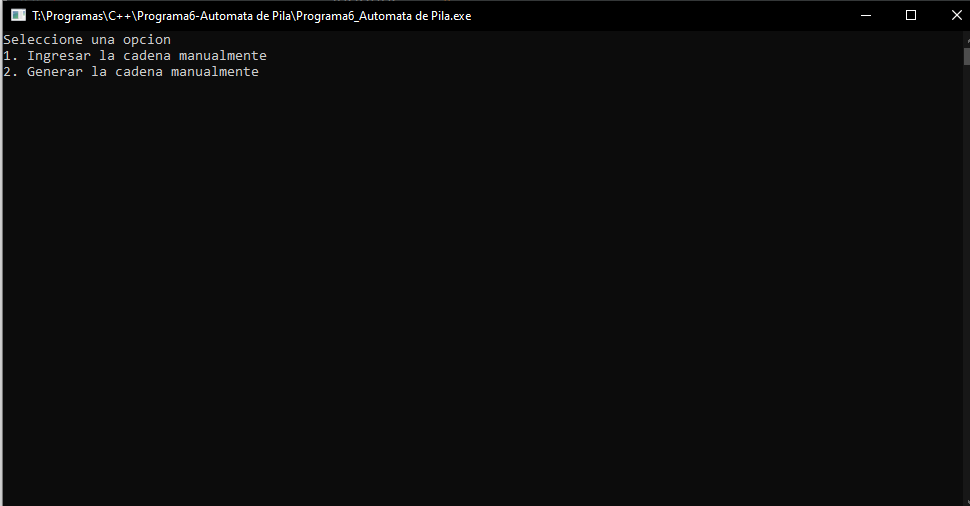
\includegraphics[width= 15cm, height= 5cm]{p6-1.png}

Cadena  = 000111- Modo Manual
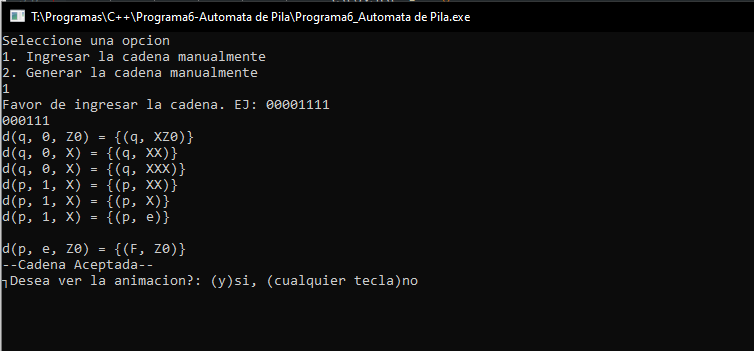
\includegraphics[width= 15cm, height= 5cm]{p6-2.png}

Cadena  = 000111- Modo Aleatorio
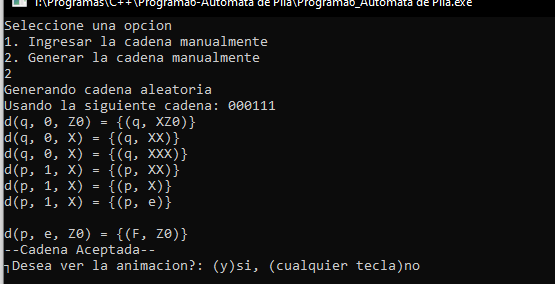
\includegraphics[width= 15cm, height= 5cm]{p6-5.png}
\newpage

Ejemplo de Animacion
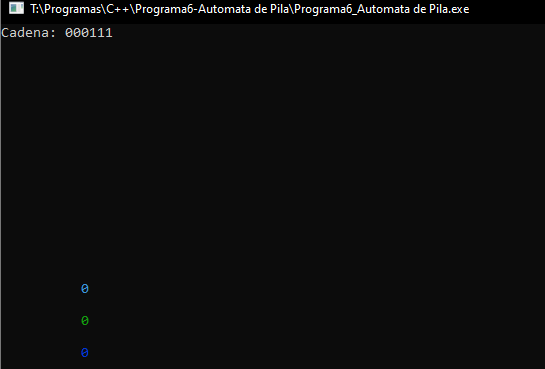
\includegraphics[width= 15cm, height= 5cm]{p6-3.png}

Final
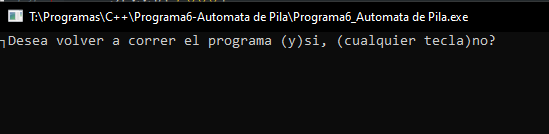
\includegraphics[width= 15cm, height= 5cm]{p6-4.png}



\end{flushleft}
\end{document}